%%%%%%%%%%%%%%%%%%%%%%%%%%%%%%%%%%%%%%%%%%%%%%%%%%%%%%%%%%%%%%%%%%%%%%%%%%%%%%%%
% Template for USENIX papers.
%
% History:
%
% - TEMPLATE for Usenix papers, specifically to meet requirements of
%   USENIX '05. originally a template for producing IEEE-format
%   articles using LaTeX. written by Matthew Ward, CS Department,
%   Worcester Polytechnic Institute. adapted by David Beazley for his
%   excellent SWIG paper in Proceedings, Tcl 96. turned into a
%   smartass generic template by De Clarke, with thanks to both the
%   above pioneers. Use at your own risk. Complaints to /dev/null.
%   Make it two column with no page numbering, default is 10 point.
%
% - Munged by Fred Douglis <douglis@research.att.com> 10/97 to
%   separate the .sty file from the LaTeX source template, so that
%   people can more easily include the .sty file into an existing
%   document. Also changed to more closely follow the style guidelines
%   as represented by the Word sample file.
%
% - Note that since 2010, USENIX does not require endnotes. If you
%   want foot of page notes, do not include the endnotes package in the
%   usepackage command, below.
% - This version uses the latex2e styles, not the very ancient 2.09
%   stuff.
%
% - Updated July 2018: Text block size changed from 6.5" to 7"
%
% - Updated Dec 2018 for ATC'19:
%
%   * Revised text to pass HotCRP's auto-formatting check, with
%     hotcrp.settings.submission_form.body_font_size=10pt, and
%     hotcrp.settings.submission_form.line_height=12pt
%
%   * Switched from \endnote-s to \footnote-s to match Usenix's policy.
%
%   * \section* => \begin{abstract} ... \end{abstract}
%
%   * Make template self-contained in terms of bibtex entires, to allow
%     this file to be compiled. (And changing refs style to 'plain'.)
%
%   * Make template self-contained in terms of figures, to
%     allow this file to be compiled. 
%
%   * Added packages for hyperref, embedding fonts, and improving
%     appearance.
%   
%   * Removed outdated text.
%
%%%%%%%%%%%%%%%%%%%%%%%%%%%%%%%%%%%%%%%%%%%%%%%%%%%%%%%%%%%%%%%%%%%%%%%%%%%%%%%%

\documentclass[letterpaper,twocolumn,10pt]{article}
\usepackage{usenix2019_v3}

% to be able to draw some self-contained figs
\usepackage{tikz}
\usepackage{amsmath}

\usepackage{listings}
\usepackage{parcolumns}
\usepackage{graphicx}
\usepackage{caption}
\usepackage{subcaption}
\usepackage{cleveref}

% Comment macros
\newcommand{\pra}[1]{\textcolor{blue}{\textbf{PS:} #1}}
\newcommand{\mat}[1]{\textcolor{red}{\textbf{Mat:} #1}}
%-------------------------------------------------------------------------------
\begin{document}
%-------------------------------------------------------------------------------

%do not want date printed
\date{}

% make title bold and 14 pt font (Latex default is non-bold, 16 pt)
\title{\Large \bf TikTok: Kernel TOCTTOU Protection}

%for single author (just remove % characters)
\author{
{\rm Eric Tusso}\\
EPFL
\and
{\rm Yamaha Priest}\\
EPFL
% copy the following lines to add more authors
% \and
% {\rm Name}\\
%Name Institution
} % end author

\maketitle

%-------------------------------------------------------------------------------
\begin{abstract}
%-------------------------------------------------------------------------------
Your abstract text goes here. Just a few facts. Whet our appetites.
Not more than 200 words, if possible, and preferably closer to 150.
\end{abstract}

% Talk about the system call filters and how they can be used for good
% Introduce the main problem - TOCTTOU
% Brag how our system is the best thing since sliced bread
\section{Introduction}

%\mat{Start with one paragraph motivation/setting the scene.}

%\pra{You jump straight into introducing system call wrappers. Maybe preface
%this with a para detailing how system call execution model can be exploited in
%various scenarios. After that, you can jump into how wrappers try to address the
%problems you introduced first. It'd make for a smoother transition IMO.}

Userspace programs communicate with the operating system using system calls.
System calls may contain vulenerable code that a malicious user (adversary,
attacker) can exploit to gain privileged access. When such a vulnerability
is found, it is patched, and the kernel (module) is updated. Unfortunately,
many legacy and embedded devices rely on drivers distributed as binary blobs,
compiled against a specific kernel version.

\emph{System call wrappers} enable administrators to define system call
execution policies. Such policies (\emph{filters}) prevent an execution of a
system call based on the ID of the call and its arguments. By setting only
necessary access policies for all processes, administrators reduce the damage in
case of an attack. 

%\mat{Would is not a good verb. Aim for clear statements.}
Filtering also restricts access to the exploitable system
calls. By excluding some combinations of arguments, the administrator can 
mitigate certain vulnerabilities until a patch is available. On legacy systems,
this approach can be used as a mitigation for vulnerabilities.
%\mat{Same for could. Make absolute statements, not relative ones if possible.}

%\mat{Don't use forced newlines. Ever.
%\\
%\\
%}

%\pra{You started with
%`wrappers have a design flaw` and then started talking about filters.  
%Disambiguate between wrappers and filters and maintain
%consistent terminology throughout.}

Unfortunately, system call wrappers suffer from a design flaw. They execute before system calls. After
the filter reads arguments and validates them, the system call reads them the
second time. In-between these two reads, the attacker can change values,
leading to an execution of a forbidden call. This is called a
\emph{time-of-check to time-of-use} attack (TOCTTOU). It is a consequence of a
\emph{double-fetch} from the user-space.

Double-fetches occur when a higher-privileged code (e.g. the kernel) reads
the same data twice from the lower-priviliged space (e.g. userspace). In-between
the two reads, the data can be changed concurrently. Double-fetches are then
a type of a \emph{race condition} between the two threads of different priviliges.
TOCTTOU occurs when the first read is used in a check, while the second one is
consumed by the code. 
%\pra{When? Clarify change between the double-fetch.}.
%\mat{We call it user-space, not userland.}

%\mat{Make problems explicit and enumerate them.}

The system that mitigates double-fetches needs to:
\begin{enumerate}
  \item Prevent the change of the user memory accessed by the system call
  \item Enable normal system call execution
  \item Enable normal execution of threads trying to change the arguments
\end{enumerate}


\begin{figure}[]
  \centering
  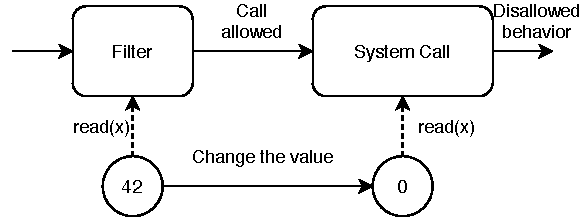
\includegraphics[width=.85\linewidth]{img/tocttou.pdf}
  \caption{Bypassing a system call filter using a TOCTTOU attack}
  \label{fig:tocttou}
\end{figure}

The double-fetch in a system-call can only be exploited by overwriting the
arguments during the call's execution. Considering that the Linux kernel uses a
well defined interface for reading from the userspace
(\texttt{copy\_from\_user}), it can be extended to mark the memory page with the
read data. If those pages are marked as read-only for the duration of the call,
double-fetches are \emph{completely eliminated}.

Writes to the marked pages are handled depending on where they come from. Writes
from the kernel go through the well defined interface (\texttt{copy\_to\_user}).
They are saved and executed at the end of the call. Writes from the userspace
will trigger a \emph{page-fault handler} where they will wait for the unmarking.

For such a memory-marking system to introduce deadlocks into software,
extraordinary conditions need to be met. The software needs to
share the \emph{same data} between threads using the \emph{shared memory} and 
\emph{message-passing} at the \emph{same time}.
%\pra{Before stating the contributions, insert a couple of paras detailing how you
%address the problem and then introducing your framework. Then you should give a peek
%into the results of your framework evaluation.}

We present \emph{TikTok} - a memory marking extension to the Linux kernel. TikTok
provides system-calls with a checkpointed view of the memory at the time they
have been read the first time. This mitigates not only the double-fetch bugs
which can be fixed, but also the ones which are there by design (e.g. system-call
wrappers). TikTok works on modern Linux distributions (Ubuntu Server 18.04 LTS)
and doesn't require any modifications to user programs. TikTok isn't suitable
for servers and highly multithreaded workloads, but can be used on embedded
devices.

The main contributions of this paper are:
\begin{itemize}
\item TikTok - mitigation for the time-of-check to time-of-use attacks on system 
      call arguments in the Linux kernel
\item A technique to postpone the writes to marked pages from userspace
\item A technique to defer the writes from the kernel to the marked pages,
      while continuing the execution of the system call
\end{itemize}



%\pra{This seems out of place. Each section would have a lead introducing its purpose
%so this is redundant information.}
%\mat{Each systems paper has the same outline. This paragraph can be removed without loss of information.}
%The rest of the paper is organized as follows: \Cref{sec:background} explains 
%inter-process communication, paging, double-fetch bugs, and the related
%background. \Cref{sec:design} describes how \emph{TikTok} works in theory, while
%\cref{sec:implementation} elaborates on the x86-64 implementation. Related work
%is discussed in \cref{sec:relatedwork}.

% Cover the theory needed to understand how and why TikTok works
% 1) IPC - We need this to argue why the deadlocks are almost impossible
% 2) VM and Page Tables - Why it exists and how it works
% 3) x86 Page Tables - Continue the discussion from the previous section
% 4) Page faults - Explain how and why they happen.
% 5) Copy to/from user - Explain why the API has been introduced
% 6) Double-fetches - Provide a high-level overview
\section{Background}
\label{sec:background}
%\mat{What kind of message do you want to send? Why do we need this background information? Guide the reader in understanding what is necessary and where the problems are.}

%\pra{Insert lead para giving overview of info presented here as you did in the intro.}
%\pra{In its current state this section looks like an information dump. For each subsection
%in bg give context to the user as to why its relevant for TikTok.}
\Cref{subsec:ipc} introduces two different ways of communication between
processes - \emph{shared memory} and \emph{message-passing}. TikTok affects both
of these methods because the arguments of the message-passing system calls are
stored in (potentially shared) memory. This introduces additional
synchronization points when writing to them. 

\Cref{subsec:vm} covers how memory is organized on modern computers and how
permissions are implemented. The virtual memory on x86 processors is described
in \cref{subsec:x86pgtables}, followed by the handling of page faults in
\cref{subsec:pagefaults}. These sections discuss the memory protection
mechanisms used by TikTok.

The API that Linux uses to access the userspace memory and which TikTok extends is
described in \cref{subsec:copy}. \Cref{subsec:doublefetch} details the
double-fetch bugs TikTok is mitigating.

\subsection{Interprocess Communication}
\label{subsec:ipc}

The two main types of communication between processes are \emph{shared memory} 
and \emph{message passing}\cite{silberschatz2018operating}.

Shared memory relies on two processes having a section of memory that both can 
access. Data transfer is fast, but the synchronization is problematic. 
Processes must monitor shared memory for changes, leading to unnecessary
polling.

Message passing consists of one process calling send, and another one calling
receive to fetch the message. Synchronization is guaranteed, with parties
waiting for their calls to be served. However, unnecessary message copying can
occur between processes on the same system.

Modern operating systems support both of these approaches. The downsides are
usually offset by adding the  bare minimum of the other approach (e.g. shared
memory with semaphores, or message passing with shared buffers). Two processes
usually use only one paradigm to communicate. Sending messages and writing
to the shared memory at the same time is exceptionally rare.

\subsection{Virtual Memory and Page Tables} \label{subsec:vm}

Operating system (OS) provides an illusion that every process is executing alone
on the processor. To accomplish this, the OS needs to restore the program state
on the context switch between two processes (e.g. CPU registers) and to prevent 
processes from accessing each other's memory. Memory is protected by
\emph{virtualization}. Processes use \emph{virtual addresses} that get mapped to
the \emph{physical addresses}. When the OS moves data to a different physical 
address, the virtual address referring to the data remains the same.

Virtual memory can be implemented by storing different processes' data at 
different offsets in physical memory and limiting the access to corresponding 
memory chunks. Each process's memory chunk is called a segment and the 
implementation is called \emph{segmented virtual memory}. The translation is 
accomplished by adding an offset to the virtual address. Considering that 
segments need to be continuous, the free physical memory can be fragmented
such that the OS cannot find a part large enough to store a new process.

\begin{figure}

  \begin{subfigure}[]{.45\linewidth}
    \centering
    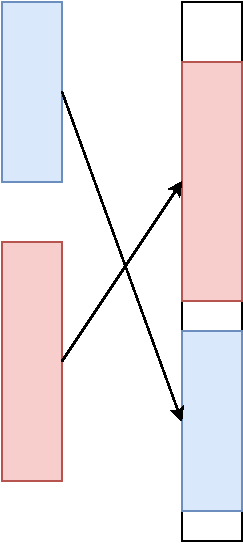
\includegraphics[width=.5\linewidth]{img/segmented.pdf}
    \caption{Segmented}
  \end{subfigure}
  \hfill
  \begin{subfigure}[]{.45\linewidth}
    \centering
    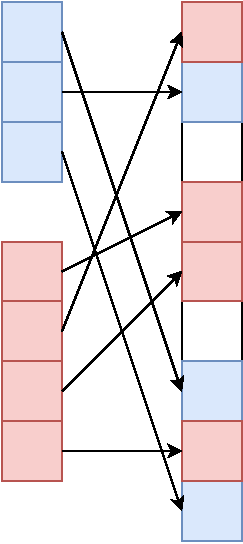
\includegraphics[width=.5\linewidth]{img/paged.pdf}
    \caption{Paged}
  \end{subfigure}

  \caption{Two virtual memory spaces mapped to physical memory using segmented
  and paged approaches}
\end{figure}

\emph{Paged virtual memory} is more flexible. The physical memory is partitioned
into fixed-size pages (usually 4 kB). A page in the virtual memory space gets
mapped to the corresponding page in the physical memory. The mapping function is
defined for each process by a \emph{page-table}. Page-tables store the reference
to the mapped physical memory (\emph{page frame}). They also keep
the access permissions for each page (\emph{read}, \emph{write}, \emph{execute},
 \emph{user}, \emph{superuser}). In case of low memory, rarely accessed pages 
can be moved to the disk, and replaced by immediately needed pages. This process
is called \emph{swapping}. Similarly, when processing a file, pages do not need 
to be loaded immediately, but on the first access (\emph{on-demand paging}). The
\emph{present} bit is added to differentiate between present and absent pages.

Virtual memory spaces are quite large ($2^{64}$ bytes on a 64-bit processor). A 
table containing all one-to-one mappings would be impossibly large to store. 
Page tables are therefore stored as trees with only the allocated memory being 
present (\cref{fig:pagetable}). However, instead of just reading the 
corresponding physical address on memory access, the processor now needs to 
perform a tree traversal. Different bits in a virtual address encode the path 
the processor needs to take to obtain the page frame number (e.g. the first 8 
bits tell CPU which entry on the first level it needs to dereference). Traversal
needs to be fast. It is implemented in hardware by the \emph{memory management 
unit} (MMU). Reading the page table from memory is slow, so a small cache is 
added to the MMU to store frequently accessed page entries - 
\emph{translation-lookaside buffer} (TLB). On modern processors, TLB consists of
several levels, and can even be backed by another MMU cache. 

\subsection{x86-64 Page Tables}
\label{subsec:x86pgtables}
\begin{figure}[]
  \centering
  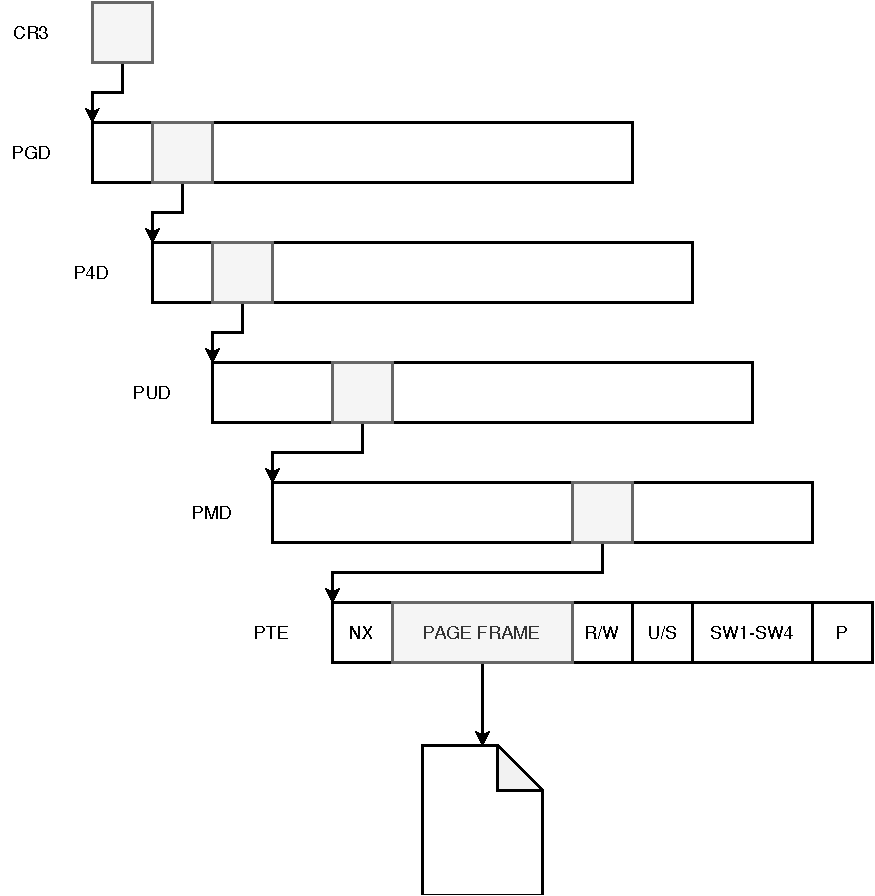
\includegraphics[width = .35 \textwidth]{img/pagetable.pdf}
  \caption{Page Table Structure on x86. Only relevant data has been included.}
  \label{fig:pagetable}
\end{figure}
x86-64 architecture officially supports paged virtual memory model with a 5 
level page table (\cref{fig:pagetable}):
\begin{description}
    \item[PGD] Page Global Directory
    \item[P4D] Page Fourth-level Directory
    \item[PUD] Page Upper Directory
    \item[PMD] Page Middle Directory
    \item[PTE] Page Table Entry
\end{description}

Every level corresponds to 8 bits in the virtual address, with the remaining 12
bits identifying the offset in the actual page frame. A page table entry
includes the following information:
\begin{description}
    \item[Present bit (\textbf{P})] is set if the page is present in memory
    \item[Read/Write bit (\textbf{R/W})] denotes if the page is writable or just
         readable
    \item[User/Superuser bit (\textbf{U/S})] represents if the page can be 
    accessed by the user, or only by the superuser
    \item[Not Executable bit (\textbf{NX})] is set if the code stored on the 
    page cannot be executed
    \item[Page Frame Number] denotes the page frame the entry points to
    \item[\textbf{SW1-SW4}] Four bits free for the OS to use
\end{description}

\subsection{Page-Faults}
\label{subsec:pagefaults}
On invalid access (e.g. wrong permissions, page not present) the MMU will
trigger a page-fault. The fault is a synchronous interrupt that executes in the
context of the faulting (accessing) thread. The page-fault handler loads an
absent page from the disk. In the case of a write to a temporarily shared page,
it creates an independent, separate copy of the page (\emph{copy-on-write}). On
permission iolation, the page-fault handler kills the thread. After the fault
finishes executing, the faulting instruction is re-executed. 

With the advent of cloud computing, user-space page-fault handling has been added 
to the Linux kernel. Users can define their routines to load swapped-out data.
This is particularly useful on computer farms when migrating virtual machines
between physical nodes. One only needs to migrate the code that is executing.
Accesses to the unmigrated memory will be passed to the user-space page-fault
handler. It will then fetch them over the network and continue the execution.

\subsection{Copy-from-User and Copy-to-User}
\label{subsec:copy}
Linux uses swapping only for user memory. When executing in the kernel context,
kernel memory is mapped and present. A page fault on kernel memory access is
therefore considered fatal. However, the kernel needs to access potentially
paged-out user memory. The user memory is also limited to the lower half of the
virtual memory space. On every access to the user-pointer, the kernel needs to
verify this constraint.

Linux provides functions and macros for user-memory access from the kernel to 
enforce the checks. A page-fault generated by them is treated as a fault in the
user process which had invoked the executing system call.

%\pra{This looks very space inefficient formatting.
%Tabular environment or just in plaintex would conserve more space.}:
The interface for communication with userspace: \texttt{(\_\_)copy\_(from/to)\_user},
\texttt{(\_\_)(get/put)\_user}, \texttt{user\_str(cpy/len)}.
BSD also provides a similar interface using \texttt{copy\_in} and 
\texttt{copy\_out} functions.

\subsection{Double Fetch Bugs}
\label{subsec:doublefetch}

\begin{figure}[]
  \centering
  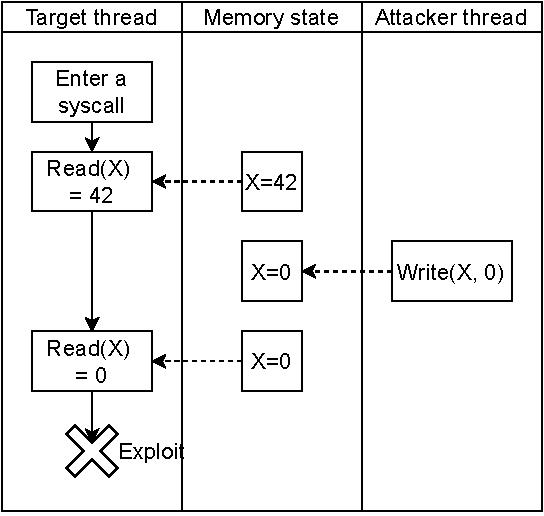
\includegraphics[width=.85\linewidth]{img/doublefetch.pdf}
  \caption{Diagram of a double-fetch bug}
  \label{fig:doublefetch}
\end{figure}

\emph{Double-fetch} bugs occur when a privileged environment (such as the 
kernel) reads untrusted memory two or more times (\cref{fig:doublefetch}). 
In between those two reads, memory could have been changed by an unprivileged
adversary. Considering that this bug relies on carefully timed accesses
for two different threads, it is a variant of a race condition. The situation
where the first fetch validates the value of the fetched variable, 
but the computation is only performed on the second fetch, is called a 
\emph{time-of-check to time-of-use} (TOCTTOU) bug. TOCTTOU bugs have been
widely studied in file systems, where the API makes it possible to swap the file
after validating the access rights \cite{payer2012protecting,
pu2006methodical, wei2010modeling, tsafrir2008portably}.


Wang et al. explain in \cite{wang2018survey} that double-fetches appear not only
in kernels, but wherever there is a trust boundary to cross (e.g. kernel -- 
hypervisor, hardware -- kernel). Double-fetches have been responsible for many
vulnerabilities in the kernel.

% Explain generally how TikTok works. We mention all the problems that
% TikTok needs to mitigate: writes from user-space, writes from the kernel, safely
% stopping the writes, preventing bypass using file-backed pages, system calls
% that are ignored. The most important part is showing the conditions for 
% introducing deadlocks
\section{Design}
\label{sec:design}
%\pra{This section does not really look like a "high-level overview" but more like
%the detailed design itself. :) I would suggest having a separate overview subsection that summarizes
%the main design points.}
%\mat{Style: don't write 'in this section'. It's obvious that it's in this section, so you're just wasting space.}

%\pra{A general comment on the design. Currently, it reads more like a tutorial about
%a cool framework rather than an actual design. All the necessary information required to
%create a design section is here, it just needs to presented better and in a more structured
%way.:) 
%As a suggestion, I think in this section you should first enumerate all possible attack vectors
%for an adversary trying to mount a toctou attack and then present your design policies(3.2, 3.3, 3.5 and 3.6) and
%how they address those attack vectors. IMO the deadlock issue (3.4 and 3.7) is something that 
%needs to be discussed separately since it is not a part of your actual design but moreso
%a consequence of your design.}
%\mat{Agreed with Prashast}
\subsection{Overview}
\label{subsec:designoverview}
TikTok protects the pages storing the buffers by marking them
read-only. The capabilities of the attacker trying to bypass these measures
are described in \cref{subsec:secmodel}.

TikTok needs to protect the buffers from different types of attacks:

\begin{enumerate}
  \item \label{first} Writes from the userspace
  \item \label{second} Writes from the kernel
  \item \label{third} Bypassing TikTok by mapping file-backed pages as writable
  \item \label{fourth} Bypassing TikTok by using a write call to change file-backed pages
  \item \label{fifth} Bypassing TikTok by mapping device-backed files
\end{enumerate}

All of these potential vulnerabilities have been noticed by Watson when he
analyzed CerbNG\cite{watson2007exploiting} and other system call wrappers.
TikTok must ensure that the protections don't interfere with the correct
execution of the kernel and user programs. In other words - both writes and the
execution flow can only be temporarily affected.

The paradox of memory marking schemes can be seen in the case of system calls
that both read and write to the user memory (e.g. \texttt{rt\_sigaction}).
Simply marking the pages as read-only prevents attacks from the userspace, but
also stops the system call from performing the required write. However, if one
enables the writes for the kernel, the adversary can bypass the protection
using a simple \texttt{sys\_read} call to the marked page.

The protection against the attacks \ref{first} and \ref{second} are described in
\cref{subsec:memorywrites}. The defenses against \ref{third}, \ref{fourth}, and
\ref{fifth} are discussed in \cref{subsec:filewrites}.


\subsection{The Security Model}
\label{subsec:secmodel}
The administrator has set up \emph{Descretionary Access Control} (\emph{DAC})
that can prevent the adversary from accessing certain files. They also control
which file-systems are mounted on the machine and have disabled user-space
page-fault handling.

The adversary has access to a user account on a target machine. They can execute
arbitrary code (including system call) and want to obtain root access by 
triggering a TOCTTOU bug in the kernel.

\subsection{System Call Argument Protection}

\label{subsec:memorywrites}
\begin{figure}[]
  \centering
  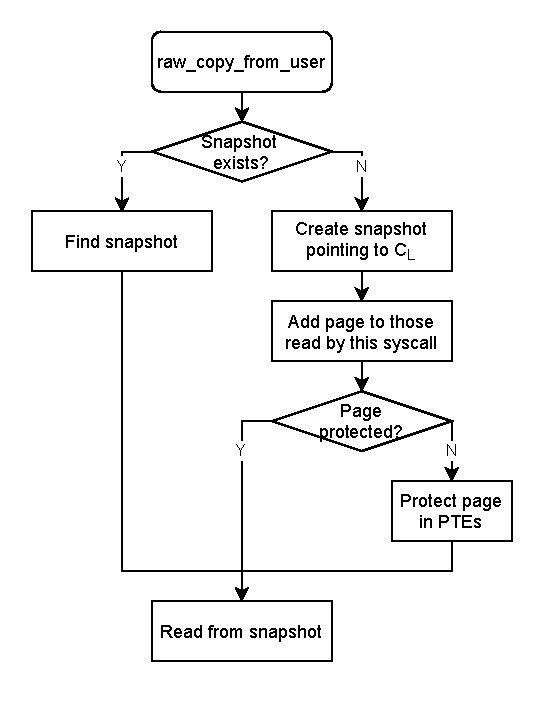
\includegraphics[width = .45 \textwidth]{img/copy_from_user.pdf}
  \caption{\texttt{copy\_from\_user} marks both the file and the pages before
  reading in the data}
  \label{fig:copyfromuser}
\end{figure}

%\pra{I think 3.2 and 3.3 can be merged together into something named along the
%lines of "System Call Argument protection" subsection. The lead for this merged
%section should use threat model as motivation to show that syscall arugments can
%be manipulated from both user and kernel space by adversary. Then, you should
%detail how TikTok handles them as explained below.} 
Defending against the writes from userspace (\cref{first}) is the primary
feature of TikTok. System calls read user memory using \texttt{copy\_from\_user}
and its variants. Calls to \texttt{copy\_from\_user} mark the pages as
\emph{read-only} in all virtual memory spaces mapping it
(\cref{fig:copyfromuser}). Multiple system calls can mark a page at the same
time. The benefit of marking the page this way is that it can still be read by
other user threads, reducing the negative effects of TikTok. When all the system
calls that use the page finish executing, the page is \emph{unmarked} -- the
previous permissions are restored.

However, marking the pages is the first part. TikTok needs to guarantee that the
programs will still execute correctly. Userspace writes to the marked pages
trigger a page-fault (\cref{fig:pagefault}). In the page-fault handler TikTok
intercepts these writes and stops them until the page has been unmarked. After
the unmarking, the thread will exit the handler and redo the write. This
technique introduces additional synchronization points for concurrent programs.
Combined with the coarse granularity of pages (4KBs) deadlocks come up as a
potential problem. They are discussed in \cref{sec:deadlocks}.

\begin{figure}[]
  \centering
  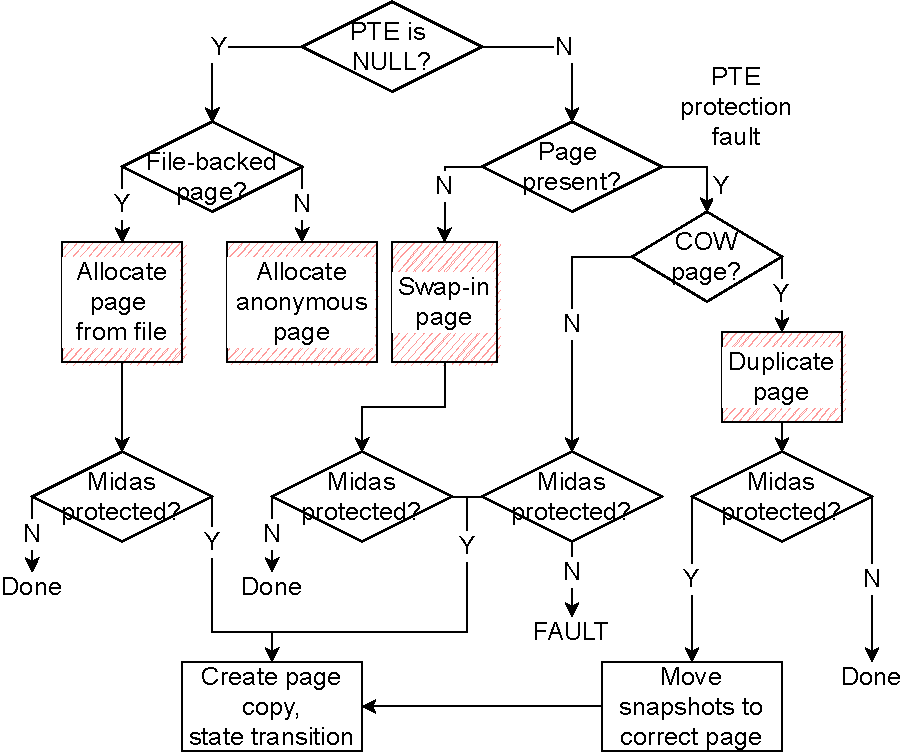
\includegraphics[width = .75 \linewidth]{img/pagefault.pdf}
  \caption{TikTok's handling of the writes to a marked page}
  \label{fig:pagefault}
\end{figure}

\subsection{Protecting System Call Arguments from Writes by the Kernel}
\label{subsec:kernelland}
\begin{figure}[]
  \centering
  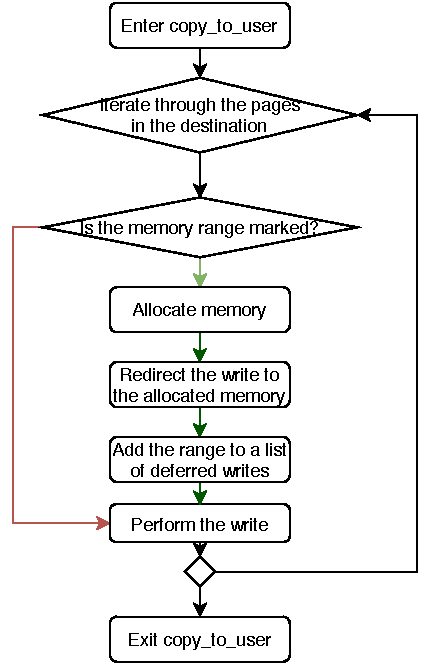
\includegraphics[width = .30 \textwidth]{img/copy_to_user.pdf}
  \caption{\texttt{copy\_to\_user} defers the writes from kernel until the end
  of the system call}
  \label{fig:copytouser}
\end{figure}

The process that stops the userspace writes cannot be applied to the writes from
the kernel (attack \ref{second}). As mentioned in \cref{subsec:designoverview},
such a system would self-deadlock after a system call performs a read and a
write to the same page (\texttt{rt\_sigaction}). Any solution involving giving
the write permissions to the kernel results in the adversary bypassing the
marking using a system call (e.g. \texttt{sys\_read}).

Unlike userspace writes to user memory, which can happen from any place in the
code, kernel writes can only take place from \texttt{copy\_to\_user} and its
variants. TikTok uses this to its advantage. When the kernel uses
\texttt{copy\_to\_user} to write to a marked page the write is \emph{deferred}
until the end of the call. The function \texttt{copy\_to\_user} exits normally
with the data saved into a data structure. This prevents self-deadlocks because
the program continues the normal execution. At the end of the call (\emph{after
unmarking}), the writes are performed from the data structure in the order in
which they arrived. If the pages are still marked, the writes will wait just
like the writes from userspace.

These two techniques create a snapshot of the memory at the moment it
was accessed for the first time. This means that all reads will always return
the original values, even if call had written to them in-between. In case a
system call performs a re-read of the location it has written to and expects a
new value, TikTok would return the old one. However, the authors haven't
encountered such a case, and TikTok can be easily extended to support it.

Unfortunately, some system calls rely on writes from userspace for some of their
functionality. \texttt{pollfd}\cite{pollfd} loops through an array of structures
to check if any of the files are ready to perform I/O. Writing -1 to one of the
fields makes the system call ignore that descriptor. \texttt{futex}\cite{futex}
is a userspace variant of the mutex. Marking a page in the \texttt{futex} call
would result in the userspace thread not being able to unlock it and a deadlock.
TikTok ignores such calls --  they expect the writes from the userspace.

Another reason to ignore system calls is performance. Certain calls may have
buffer arguments, but the data is \emph{unformatted}. Unformatted data is
essentially an array of bytes. Overwriting this data is equivalent to passing
different data to the call. Considering that the \texttt{write} call takes
unformatted data as one of its arguments, this frequently called interface does
not need to be protected.


\subsection{Protecting Against File-Based Attacks}
\label{subsec:filewrites}
Memory in Linux can be \emph{file-backed} and \emph{anonymous}. File-backed 
pages have map to a corresponding file. Anonymous pages do not have a backing 
file (e.g. stack and heap).

Another classification is based on privacy: \emph{private} and \emph{shared}. 
Private memory is part of only one virtual memory space. This memory space can 
be accessed by multiple threads in a process, but no threads outside the process
have access. Shared memory can be accessed by multiple processes.

\begin{table}[]
  \begin{tabular}{|l|l|l|}
  \hline
          & Anonymous         & File-backed                           \\ \hline
  Private & /                 & Copy-on-write                         \\ \hline
  Shared  & Inherited by fork & Can be (un)mapped at any time         \\ \hline
  \end{tabular}
  \caption{Properties of the different types of memory in Linux}
  \label{tab:memory}
\end{table}

Unlike private memory and shared anonymous memory, shared file-backed memory can
be mapped and unmapped at will (\cref{tab:memory}). It also preserves its state
when unmapped. This enables an adversary to map a marked page as writable and
edit it (attack \ref{third}). TikTok intercepts the mapping of memory and checks the
page frames being mapped. The pages are then mapped with appropriate permissions
into the virtual memory space.

Files in Linux can be accessed in two ways:
\begin{itemize}
    \item by mapping the file to memory
    \item by using system calls to modify the file (e.g. \texttt{write})
\end{itemize}

Watson has noticed that protected file-backed pages could still be edited by a
\texttt{write} call (attack \ref{fourth}). The mapped memory would reflect the state
of the file and result in changed values. TikTok prevents this attacks by
pausing the write to the corresponding file as long as it has any marked mapped
pages. The implications of this for deadlocking are discussed in
\cref{sec:deadlocks}. 

Devices are treated as files in Linux and can be memory mapped. However, 
hardware may change its registers at will. There are no conceivable ways from 
protecting from TOCTTOU attacks if the adversary stores his arguments in device
mapped memory. Considering that mapping device memory to user-space is considered
bad practice, we rely on \emph{Descretionary Access Control} (\textbf{DAC}) to 
prevent users from mapping devices in the first place (attack \ref{fifth}).


\section{TikTok Deadlocks}
\label{sec:deadlocks}

\Cref{sec:design} mentions that TikTok may introduce deadlocks to valid
programs. For an OS extension even a small chance of a random deadlock violates
the presumption of correctness and is unacceptable. Luckily, TikTok deadlock can
happen only under specific, rare circumstances which violate the principles of
Interprocess Communication (\cref{subsec:ipc}).

TikTok adds additional synchronization points to multi-threaded programs by
stalling the writes. It is possible for these points to introduce previously
non-existent deadlocks to programs.Such deadlocking threads would need to
communicate using both shared memory (for TikTok to stop one of them) and
synchronous system calls (for TikTok to mark memory).


\begin{figure}
  \centering
  \begin{subfigure}[b]{0.45\linewidth}
  \begin{minipage}{\linewidth}
  \begin{lstlisting}
  1: S(A,T1);  
  \end{lstlisting}
  \end{minipage}
  \caption{Thread 1}
  \end{subfigure}
  \hfill
  \begin{subfigure}[b]{0.45\linewidth}
  \begin{minipage}{\linewidth}
  \begin{lstlisting}
  2: write(A);
  3: unblock_S(T2);
  \end{lstlisting}  
  \end{minipage}
  \caption{Thread 2}
  \end{subfigure}
  \caption{Executing instructions in the specified order causes a deadlock with TikTok}
  \label{fig:deadlock}
\end{figure}


\Cref{fig:deadlock} shows an example of a such communication pattern. Thread 1
enters the system call S and marks a shared page \texttt{A} (\textbf{1}). The
system call \texttt{S} blocks until the corresponding call \texttt{unblock\_S} is called
in Thread 2 (\textbf(3)). While the page \texttt{A} is still marked, Thread 2
attempts to write to it, causing it to wait for \texttt{S} to finish
(\textbf{2}). This situation is peculiar:

\begin{enumerate}
    \item The page \texttt{A} is shared between Thread 1 and Thread 2
    \item Access to page \texttt{A} is not protected by a mutex, or a semaphore
    \item System call \texttt{S} is a blocking system call that receives a 
    signal from another thread
    \item System call \texttt{S} reads its arguments from the page \texttt{A}
    \item Thread 2 needs to write to the same page where the arguments for 
    \texttt{S} are stored (page \texttt{A})
    \item Even though Threads 1 and 2 can communicate using shared memory, 
    Thread 1 needs to also invoke \texttt{S}
\end{enumerate}

Does the system call \texttt{S} even exist? A synchronization calls (locking or
signaling) are good candidate for \texttt{S}. They affect multiple threads, but
they are lightweight and their arguments are passed in registers, not in memory.
This prevents them from markings the page \texttt{A}. Message-passing system call
fits this description better. It takes arguments from memory. It can be
synchronous -- requiring the other thread to receive the message before
proceeding.

Having identified the system call \texttt{S}, the conditions for the deadlock
can be simplified to:

\begin{itemize}
  \item Threads 1 and 2 share memory (page \texttt{A})
  \item Threads 1 and 2 decide to share the data in the shared memory (page
        \texttt{A}) using message-passing
  \item Threads 1 and 2 write to the shared memory (page \texttt{A}) during the
        message-passing call                       
\end{itemize}

Programs usually rely on a single IPC apstraction (shared memory or
message-passing). Even software that uses both of them would do so for separate
functionalities. The program that replicates the communication using both
primitives would be an example of terrible programming practice. During the
testing of TikTok (\cref{sec:evaluation}) on Ubuntu Server 18.04 LTS not a
single deadlock has been encountered. While it is possible to create deadlocking
sequences, they require mixing different inter-process communication paradigms
for the same data. During testing, we have not encountered a single deadlock
caused by TikTok.

Similar sequences can be constructed using the write system call protection
presented in \cref{subsec:filewrites}. The same argument can be applied in that
case - the program needs to write to the same data to the file using both memory
mapping and a system call at the same time. We have not encountered such a
problem.


% Here we mention SOME of the interesting implementation decisions. It is
% mostly related to x86 and should be short. ARM support should also be
% be mentioned, but Future work could be a better section for that
\section{Implementation}
\label{sec:implementation}

%\mat{What's the message here? Say what you implement based on which design decisions.}
TikTok prototype has been implemented on Linux x86-64. However, TikTok can be
ported to any operating systems that use a defined interface for reads and
writes to the userspace, as well as any architecture that has page tables
encoding access control information. Depending on the available resources so
information can be stored in different places (e.g. PTE or global structures).

\Cref{fig:bookkeeping} illustrates some of the most important data structures used in the prototype.
\cref{subsec:frameinfo} describes the data about the physical page
frame with some of the limitations due to the need to keep \texttt{struct page} as small as possible.
The data stored in the page table is explained in \cref{subsec:pageinfo}.

\subsection{Storing the Page Frame Information}
\label{subsec:frameinfo}
Linux divides physical memory into page frames. Each page frame is represented
by a \texttt{struct page}. Considering that this structure is replicated
millions of times, every additional field has a tremendous impact on memory
consumption.
\\
\\
To keep the memory consumption low, TikTok uses a single bit in \texttt{struct
page} to mark page frames. Considering that x86-64 has enough bits in the flag
field, we have decided to use one of the flag bits for this purpose.
Architectures that have fewer flag bits (such as x86) can instead use some of
the bits used by other features (e.g. Kernel Shared Memory or NUMA domains). On
\cref{fig:bookkeeping} this field is denoted by \emph{Page Marked Flag}.
\texttt{struct page} also stores a pointer to the \emph{reverse mapping}
information. The reverse mapping is used to find all PTEs \emph{TikTok} needs to
(un)mark.
\\
\\
The marking metadata is stored in a hashmap based on the \emph{page frame
number}. The access to these entries is protected by separate mutexes to improve
the scalability of the system. The metadata comprise the page frame number, the
count of threads marking the page (\emph{owners}), the number of threads waiting
for the page to get unmarked (\emph{guests}), and a \emph{queue} they are
waiting on. 

\subsection{PTE Information}
\label{subsec:pageinfo}

When we mark a page we change some of the flags in the PTEs mapping it
(\cref{fig:bookkeeping}):

\begin{description}
  \item[R/W] gets set to \emph{read-only} to prevent writes to the page
  \item[SW2] gets the old value of \textbf{R/W}
  \item[SW3] gets set to 1 
\end{description}

It is interesting to note that \textbf{SW2} is used by the Software Dirty Pages
feature of Linux. This feature cannot run alongside TikTok in our prototype.
Other architectures may have less, or more bits available for the OS to use. In
the case of lack of space in the page table, \texttt{SW2} and \texttt{SW3} could
be stored in a data separate structure.

\emph{Copy-on-write} pages have a peculiar optimization. They are marked only in
the process requesting the marking. Writes from other processes will trigger a
copy-on-write mechanism, preventing them from changing the data.

TikTok does a partial flush of the TLB and updates the MMU cache to make these
changes visible immediately.

\begin{figure}[]
  \centering
  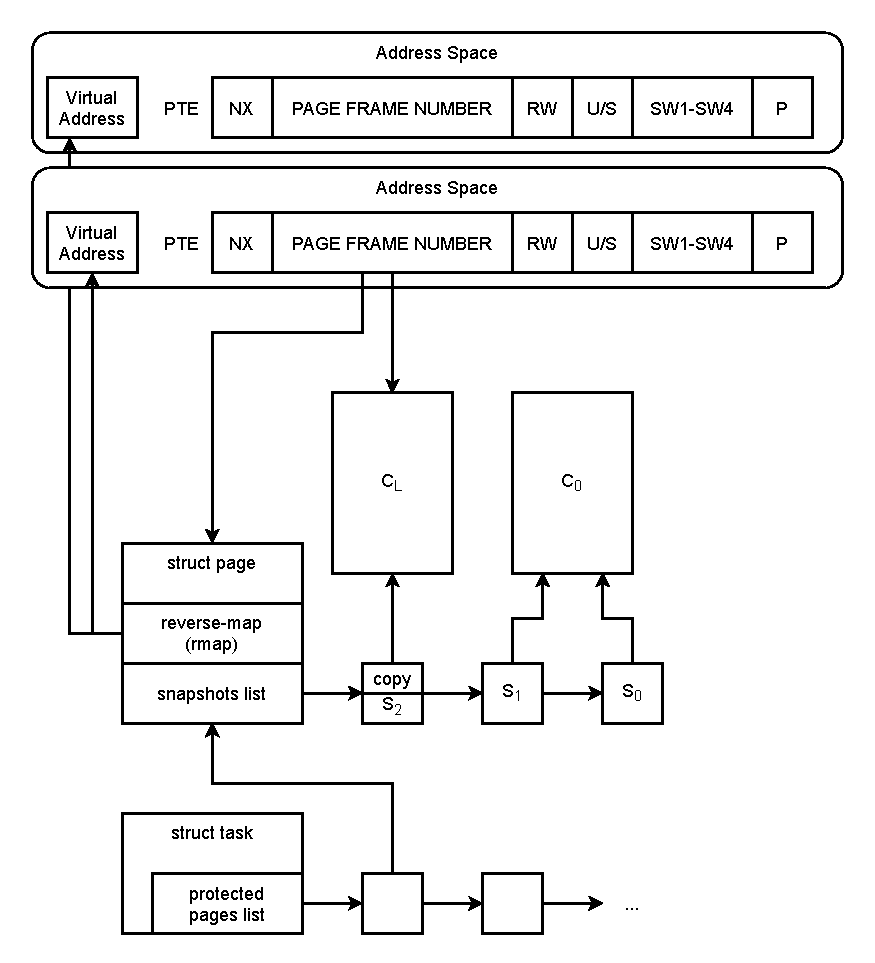
\includegraphics[width=\linewidth]{img/book-keeping.pdf}
  \caption{The most important marking information on x86}
  \label{fig:bookkeeping}
\end{figure}


% In this section we need to convince the reader in two things:
% 1) Alternative filtering approaches to system call filters are incomplete and
% cumbersome
% 2) The best way to solve the TOCTTOU bug in filters is TikTok. All other
% methods can only fix other double-fetches, or they force you to use TSX
\section{Related Work}
\label{sec:relatedwork}

%\mat{Numbers smaller than 10 should be written out: two!}
The literature related to TikTok can be broadly divided into two groups. In the
first group are system call wrappers whose main vulnerability TikTok is
mitigating. The second ones are the mitigations and solutions for
double-fetches, which are a superclass of TOCTTOU bugs.

We describe the benefits that system call wrappers compared to other solutions.
We show that all other filters that ignore or remove the TOCTTOU problem have
to either reduce the security guarantees they offer, or violate the separation
of the filter and the system call.

Afterward, we take a look at alternative ways to address the TOCTTOU bug of the
system call wrappers. Most of them are focused on finding and fixing the bug,
which isn't possible in this case. TikTok is also compared against other runtime
mitigations of double-fetches.

\subsection{System Call Wrappers and Filters}

Watson \cite{watson2007exploiting} scrutinized the security of many system call
wrappers. Not only that he found that all of them were insecure, Watson
described the different types of TOCTTOU bugs and discussed potential fixes. In
a short paragraph, he mentions that Pawel Dawidek, the creator of CerbNG
\cite{zak_frasunek_dawidek}, has experimented with marking arguments read-only.
CerbNG was an early system call filtering system for BSD that used
copy-on-read-and-write to a new memory page.

Afterward, Watson briefly discusses problems such memory marking systems
need to solve: 
\begin{itemize}
    \item unnecessary page-faults
    \item bypassing memory marking using IO system calls
    \item mapping shared memory with different permissions
    \item handling system calls that both read and write to the same memory
\end{itemize}

According to Watson, no memory-marking system (including CerbNG) addressed all
of these problems. TikTok does exactly that. Unnecessary page-faults are rare
and they are used to make the offending threads wait for unmarking. After the
page has been unmarked, the write proceeds without any consequences. Write
system call does not proceed until there are no marked pages of the file. If
needed, pages are marked when they are mapped. TikTok postpones all writes to
marked pages coming from the kernel while allowing the system calls to execute
correctly.

Modern system call wrappers can be classified into two groups, based on how they
approach the TOCTTOU attack. The first group eliminates all functionality
vulnerable to the attack. Linux's \emph{SecComp}\cite{seccomp} and
\emph{eBPF}\cite{ebpf} belong to this group. The second group moves the filter
checks deeper into the system calls, eliminating the need to read the arguments
twice. \emph{Landlock Linux} \cite{landlock} and Google's \emph{Kernel Runtime
Security Instrumentation} (KRSI)\cite{krsi} embrace this technique.

\subsubsection{Partial Solutions}
SecComp\cite{seccomp} uses \emph{Berkeley Packet Filter} (BPF) to provide small,
programmable filters that execute before the system call. Based on the values
in registers, Linux can decide whether to allow or to prevent a system call.
However, BPF cannot dereference pointers because an adversary would be able to
bypass those checks using a TOCTTOU attack. \emph{Extended Berkeley Packet
Filter} (eBPF)\cite{ebpf} provides larger filters that can also dereference
user pointers. However, eBPF cannot be used for security purposes - it cannot
stop system calls from executing. EBPF is completely read-only and can only be
used for tracing.

\subsubsection{LSM-based Solutions}
Landlock\cite{landlock} and KRSI\cite{krsi} use the \emph{Linux Security Module}
\cite{morris2002linux} (LSM) hooks to call filter checks after the arguments
have already been copied into the kernel. LSM hooks have been imagined as a set
of places where arbitrary checks can be performed before accessing a kernel
resource. Execution proceeds only if the execution has been successful.
Different security modules can provide different hooks to provide different
guarantees (e.g. \emph{SELinux}\cite{smalley2001implementing} and
\emph{AppArmor}\cite{gruenbacher2007apparmor}).

Both Landlock and KPSI attach eBPF filters to hooks, allowing users to provide
custom rules for system calls. For this solution to work everywhere for perfect
syscall filtering, LSM hooks would need to be manually added to all Linux
drivers and ioctls. Unfortunately, this is highly impractical and requires
considerable effort from a large group of developers. Considering that LSM
focuses on access control to kernel objects, it is questionable if an LSM module
can be used to mitigate bugs based on the system call arguments. Some of the
bugs could manifest themselves before a hook has been executed. TikTok is a
generic solution that does not require modifying the drivers, nor the use of
LSM hooks. Once it is deployed, all double-fetch bugs are eliminated from all
the drivers. A system call wrapper that uses TikTok can be completely
independent of the implementation of the system calls it is filtering.

\subsection{Double-Fetch Solutions}

Solutions for double-fetch bugs can be divided into \emph{static} and
\emph{dynamic} techniques. Static techniques do not execute the program but
analyze the source code. Dynamic techniques analyze the execution of the
program to find any violations.

\subsubsection{Static Analysis Work}
\label{subsec:dfstatic}
Static analysis techniques analyze the source code to find double-fetch bugs.
Wang et al. \cite{wang2017double} used pattern matching to find potential
double-fetches. They implemented a tool that patches certain double-fetches
automatically. However, their method in the general case produces false
positives that need to be inspected manually. Xu et al.\cite{xu2018precise}
improved on this work by proposing Deadline. Deadline does not use the pattern 
analysis on the source files to detect double-fetches, but a compiler's
intermediate representation and constraint solving to eliminate false positives.

Static analysis techniques such as these have the benefit of being able to find
bugs in the code that we cannot run (e.g. we are missing hardware to test the
drivers). However, they are meant for bug detection, not mitigation. Even though
the tools can fix some bugs automatically, this is not always possible. The
TOCTTOU bug is in system call wrappers by design. Double-fetches not visible in
the source, nor in the intermediate representation are another problem.
Compilers can introduce such invisible double-fetches when allocating registers
to variables. TikTok is a mitigation technique that works even in such cases.


\subsubsection{Dynamic Analysis Work}
Google Project Zero's Bochspwn \cite{jurczyk2013bochspwn} uses an emulator to
detect double-fetches. It found quite a large number of bugs in the Windows
kernel. Bochpwn works on binaries. It does not require access to the source code
and it detects bugs introduced by compilers. However, it is also limited to the
detection of double-fetches. Similarly to work presented in 
\cref{subsec:dfstatic}, developers need to manually fix the bugs. However, with
dynamic analysis a double-fetch needs to be executed, limiting this
technique to the core kernel and to the drivers with the available hardware.

A big leap in dynamic analysis techniques has been presented by Schwartz et al.
\cite{schwarz2018automated}. The first part of the paper introduces DECAF - a
framework that uses side-channel attacks to create a fuzzing oracle for
double-fetch bugs. While Bochspwn relies on emulation, slowing the execution
significantly, DECAF runs natively. It also eliminates false positives by
automatically exploiting found bugs.

Schwartz et al. then discuss a real-time mitigation technique for double
fetches - DropIt. DropIt uses Intel's \emph{Transactional Synchronization 
Extensions} (TSX)\cite{intel64and} in a creative way to prevent double-fetch
bugs. By encapsulating the code in a TSX transaction, writes from other threads
to the addresses that have been accessed will result in the
transaction being aborted. However, the code executing inside a TSX transaction
is severely limited. All reads must fit in the L3 cache, and all writes in L1.
Some instructions are also forbidden. TikTok has none of those limitations.
It works on non-Intel processors and relies on page tables for protection - a
technique that has been present for several decades.


%-------------------------------------------------------------------------------
%\section*{Acknowledgments}
%-------------------------------------------------------------------------------

%-------------------------------------------------------------------------------
\section*{Availability}
%-------------------------------------------------------------------------------

The source code of TikTok is available at LINK. It has been released under the
GNU Public Licence.

%-------------------------------------------------------------------------------
\bibliographystyle{plain}
\bibliography{\jobname}

%%%%%%%%%%%%%%%%%%%%%%%%%%%%%%%%%%%%%%%%%%%%%%%%%%%%%%%%%%%%%%%%%%%%%%%%%%%%%%%%
\end{document}
%%%%%%%%%%%%%%%%%%%%%%%%%%%%%%%%%%%%%%%%%%%%%%%%%%%%%%%%%%%%%%%%%%%%%%%%%%%%%%%%

%%  LocalWords:  endnotes includegraphics fread ptr nobj noindent
%%  LocalWords:  pdflatex acks
